%%%%%%%%%%%%%%%%%%%%%%%%%%%%%%%%%%%%%%%%%
% Arsclassica Article
% LaTeX Template
% Version 1.1 (10/6/14)
%
% This template has been downloaded from:
% http://www.LaTeXTemplates.com
%
% Original author:
% Lorenzo Pantieri (http://www.lorenzopantieri.net) with extensive modifications by:
% Vel (vel@latextemplates.com)
%
% License:
% CC BY-NC-SA 3.0 (http://creativecommons.org/licenses/by-nc-sa/3.0/)
%
%%%%%%%%%%%%%%%%%%%%%%%%%%%%%%%%%%%%%%%%%

%----------------------------------------------------------------------------------------
%	PACKAGES AND OTHER DOCUMENT CONFIGURATIONS
%----------------------------------------------------------------------------------------

\documentclass[
10pt, % Main document font size
a4paper, % Paper type, use 'letterpaper' for US Letter paper
oneside, % One page layout (no page indentation)
%twoside, % Two page layout (page indentation for binding and different headers)
headinclude,footinclude, % Extra spacing for the header and footer
BCOR5mm, % Binding correction
]{scrartcl}

%%%%%%%%%%%%%%%%%%%%%%%%%%%%%%%%%%%%%%%%%
% Arsclassica Article
% Structure Specification File
%
% This file has been downloaded from:
% http://www.LaTeXTemplates.com
%
% Original author:
% Lorenzo Pantieri (http://www.lorenzopantieri.net) with extensive modifications by:
% Vel (vel@latextemplates.com)
%
% License:
% CC BY-NC-SA 3.0 (http://creativecommons.org/licenses/by-nc-sa/3.0/)
%
%%%%%%%%%%%%%%%%%%%%%%%%%%%%%%%%%%%%%%%%%

%----------------------------------------------------------------------------------------
%	REQUIRED PACKAGES
%----------------------------------------------------------------------------------------

\usepackage[
nochapters, % Turn off chapters since this is an article        
%beramono, % /Use the Bera Mono font for monospaced text (\texttt)
%eulermath,% Use the Euler font for mathematics
pdfspacing, % Makes use of pdftex’ letter spacing capabilities via the microtype package
dottedtoc % Dotted lines leading to the page numbers in the table of contents
]{classicthesis} % The layout is based on the Classic Thesis style

%\usepackage{arsclassica} % Modifies the Classic Thesis package

%\usepackage[T1]{fontenc} % Use 8-bit encoding that has 256 glyphs

\usepackage[utf8]{inputenc} % Required for including letters with accents

\usepackage{graphicx} % Required for including images
\graphicspath{{Figures/}} % Set the default folder for images

\usepackage{enumitem} % Required for manipulating the whitespace between and within lists


\usepackage{subfig} % Required for creating figures with multiple parts (subfigures)

\usepackage{amsmath}%,amssymb,amsthm} % For including math equations, theorems, symbols, etc

\usepackage{varioref} % More descriptive referencing

%----------------------------------------------------------------------------------------
%	THEOREM STYLES
%---------------------------------------------------------------------------------------

%\theoremstyle{definition} % Define theorem styles here based on the definition style (used for definitions and examples)
%\newtheorem{definition}{Definition}
%
%\theoremstyle{plain} % Define theorem styles here based on the plain style (used for theorems, lemmas, propositions)
%\newtheorem{theorem}{Theorem}
%
%\theoremstyle{remark} % Define theorem styles here based on the remark style (used for remarks and notes)

%----------------------------------------------------------------------------------------
%	HYPERLINKS
%---------------------------------------------------------------------------------------

\hypersetup{
%draft, % Uncomment to remove all links (useful for printing in black and white)
colorlinks=true, breaklinks=true, bookmarks=true,bookmarksnumbered,
urlcolor=webbrown, linkcolor=RoyalBlue, citecolor=webgreen, % Link colors
pdftitle={}, % PDF title
pdfauthor={\textcopyright}, % PDF Author
pdfsubject={}, % PDF Subject
pdfkeywords={}, % PDF Keywords
pdfcreator={pdfLaTeX}, % PDF Creator
%pdfproducer={LaTeX with hyperref and ClassicThesis} % PDF producer
} % Include the structure.tex file which specified the document structure and layout

\hyphenation{Fortran hy-phen-ation} % Specify custom hyphenation points in words with dashes where you would like hyphenation to occur, or alternatively, don't put any dashes in a word to stop hyphenation altogether

%----------------------------------------------------------------------------------------
%	TITLE AND AUTHOR(S)
%----------------------------------------------------------------------------------------

\title{\normalfont\spacedallcaps{Self induced temperatures in Brownian motors}} % The article title

\author{\spacedlowsmallcaps{Jack Devine}} % The article author(s)

\date{\today} % An optional date to appear under the author(s)

%----------------------------------------------------------------------------------------

\begin{document}

%----------------------------------------------------------------------------------------
%	HEADERS
%----------------------------------------------------------------------------------------

%\renewcommand{\sectionmark}[1]{\markright{\spacedlowsmallcaps{#1}}} % The header for all pages (oneside) or for even pages (twoside)
%\renewcommand{\subsectionmark}[1]{\markright{\thesubsection~#1}} % Uncomment when using the twoside option - this modifies the header on odd pages
%\lehead{\mbox{\llap{\small\thepage\kern1em\color{halfgray} \vline}\color{halfgray}\hspace{0.5em}\rightmark\hfil}} % The header style

%\pagestyle{scrheadings} % Enable the headers specified in this block

%----------------------------------------------------------------------------------------
%	TABLE OF CONTENTS & LISTS OF FIGURES AND TABLES
%----------------------------------------------------------------------------------------

\maketitle % Print the title/author/date block

%\setcounter{tocdepth}{2} % Set the depth of the table of contents to show sections and subsections only

\tableofcontents % Print the table of contents

%\listoffigures % Print the list of figures

%\listoftables % Print the list of tables

%----------------------------------------------------------------------------------------
%	ABSTRACT
%----------------------------------------------------------------------------------------

\section*{Abstract} % This section will not appear in the table of contents due to the star (\section*)

Brownian motors are capable of converting chemical energy directly into work and are crucial for many biological processes. The purpose of this project is to consider the motors thermal interaction with  the environment, we want to know whether these thermal interactions will change the efficiency of the Brownian motors as compared to calculations made without considering coupling to the environment.

%----------------------------------------------------------------------------------------

\newpage % Start the article content on the second page, remove this if you have a longer abstract that goes onto the second page

%----------------------------------------------------------------------------------------
%	INTRODUCTION
%----------------------------------------------------------------------------------------

\section{Introduction}

Brownian motors are devices that can use stored energy to create directed motion, as well as being able to crank a rotor in the in the fashion of a traditional motor, they are also able to pump ions against a gradient and translocate molecules.
 
\subsection{The Smoluchowski equation coupled to the environment}

The main part of this project will be trying to understand the behavior of the coupled partial differential equations given by:

\begin{eqnarray}
J(x, t) &=& \gamma \frac{\partial}{\partial x} \left ( \frac{\partial V(x, t)}{\partial x} P(x, t) + k_B T(x, t) \frac{\partial P(x, t)}{\partial x} \right )  \\
\frac{\partial P(x, t)}{\partial t} &=& \frac{\partial J}{\partial x} \label{eqn:Smoluchowski} \\
\frac{\partial T(x, t)}{\partial t} &=& \frac{\partial}{\partial x} \left ( -\kappa q(x, t) + D \frac{\partial T(x, t)}{\partial x} \right ) \label{eqn:TemperatureEvolution}
\end{eqnarray} 

Where $P(x, t)$ is the probability density as a function of time $t$ and reaction coordinate $x$,  $\gamma$ is the friction coefficient, $V$ is the potential for the motor, $k_B$ is the Boltzmann constant, $T$ is the temperature, $\kappa$ is the thermal conductivity, $q(x, t) = \partial_x V(x, t) J(x, t)$ and $D$ is the diffusion coefficient for the temperature. Equation \ref{eqn:Smoluchowski} is called the Smoluschowski equation (need a citation here) and equation \ref{eqn:TemperatureEvolution} is the equation that governs the evolution of the temperature.
%----------------------------------------------------------------------------------------
%	METHODS
%----------------------------------------------------------------------------------------

\section{Methods}

\subsection{Finite differences}
The one dimensional equation can be solved on a discrete grid by using the finite differences method, the main idea behind this strategy is to approximate derivatives with equations of the form:

\begin{equation}
\frac{d f}{d x} \approx \frac{f(x - h) - f(x + h)}{2h}
\end{equation}

for some small $h$. The first thing to notice here is that our equation is "flux conservative", i.e. it can be written in the form 
$$ \frac{\partial P}{\partial t} = \frac{\partial J(x)}{\partial x} $$
In our case, $J(x) = \gamma \left ( \frac{\partial V}{\partial x} P + k_B T \frac{\partial P}{\partial x} \right ) $. Now we will discretize space and time, we will split time into $N$ discrete times  $T_1, T_2, ..., T_n, ..., T_N$ and space into $K$ discrete points $x_1, x_2, ..., x_k, ..., x_K$. With this, we can approximate the partial derivatives that occur in our equation, first we can approximate $\frac{\partial J}{\partial x}$ with.

$$ \left. \frac{\partial J}{\partial x} \right|_{k, n} = \frac{J_{k+1}^n - J_{k-1}^n}{2 \Delta x} + O(\Delta x^2) $$

And we can approximate $\frac{\partial P}{\partial t}$ with

$$ \left. \frac{\partial P}{\partial t} \right|_{k, n} = \frac{P_k^{n+1} - P_k^n}{\Delta t} + O(\Delta t) $$

We would like to have the equation involving $J$ written in terms of $P$, by propogating these derivatives through the definition for $J$ we get.

$$ \frac{P_k^{n+1} - P_k^n}{\Delta t} = \frac{1}{2 \Delta x^2} \left (P_{k+1}^n(V_{k+2} - V_{k+1}) + k_B T(P_{k+2}^n - P_{k-1}^n + P_k^n - P_{k-1}^n) - P_{k-1}(V_k - V_{k-1}) \right ) $$

Solving for $P_k^{n+1}$ gives

$$ P_k^{n+1} = \frac{\Delta t}{2 \Delta x} \left (P_{k+1}^n(V_{k+2} - V_{j+1}) + k_B T(P_{k+2}^n - 2P_{k-1}^n + P_k^n) - P_{k-1}^n(V_j - V_{k-1}) \right ) + P_k^n $$

If we write 
\subsection{Stochastic methods}
We can simulate the path of a single particle by using stochastic methods to solve the Langevin equation. By simulating many times we should be able to recover the distributions that were found through finite differencing. When simulating the system  at the microscopic level, equation \ref{eqn:Smoluchowski} becomes

\begin{equation}
d X_t = \mu(x, t) X_t + \frac{1}{2} \sigma(x, t)^2  d W_t
\end{equation}

Where $W_t$ is called a Wiener process.

%----------------------------------------------------------------------------------------
%	RESULTS
%----------------------------------------------------------------------------------------
\section{Results}
Here we will show some results of finite differencing and of the stochastic methods. Figure~\ref{fig:FiniteDifferences} shows a simulation of a particle density for a certain amount of time.

\begin{figure}[tb]
\centering 
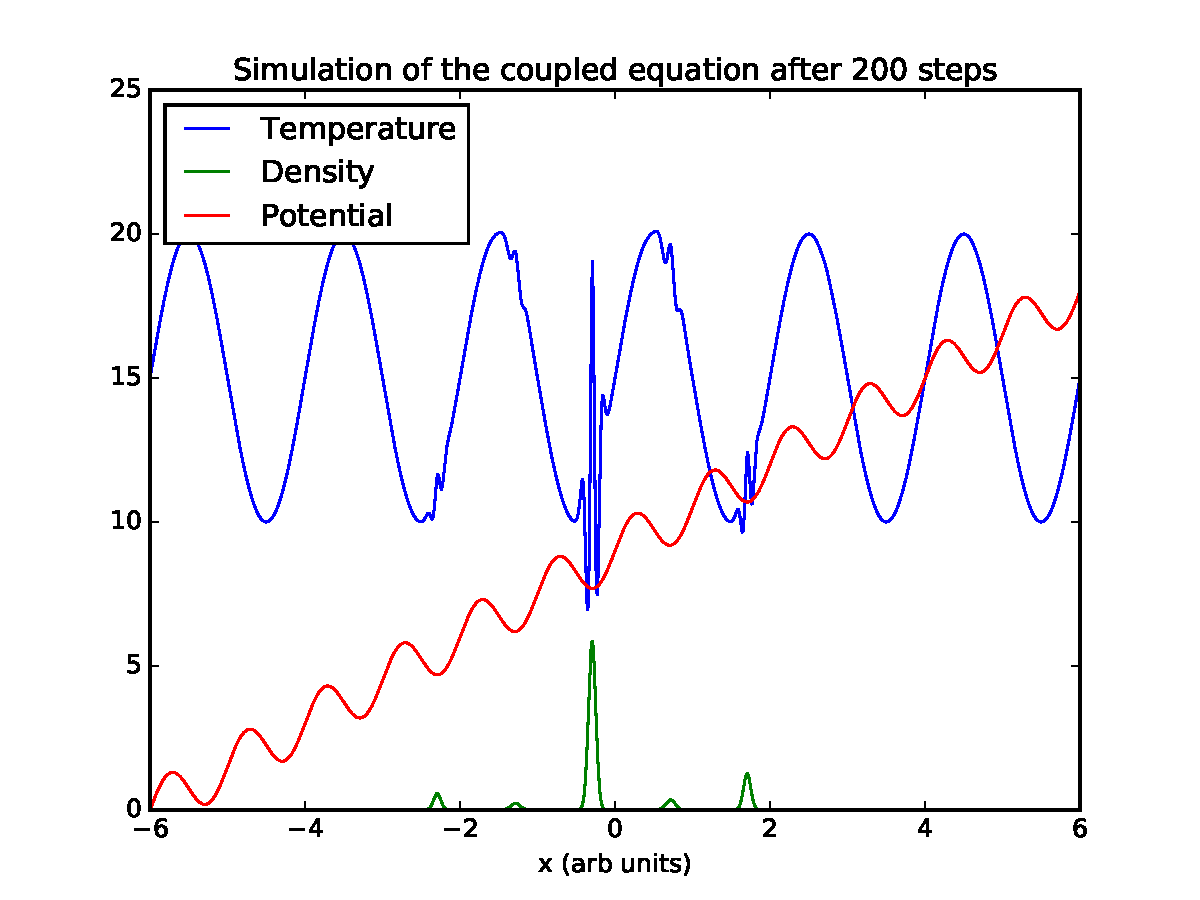
\includegraphics[width=\columnwidth]{CoupledEquationFiniteDifferences} 
\caption{Finite differencing simulation of a distribution of particles, we see that the particles are locally interacting with the environment thermally.}
\label{fig:FiniteDifferences} 
\end{figure}


%------------------------------------------------

%----------------------------------------------------------------------------------------
%	RESULTS AND DISCUSSION
%----------------------------------------------------------------------------------------

%------------------------------------------------

\cite{BlickleBechinger2011}

%------------------------------------------------

%----------------------------------------------------------------------------------------
%	BIBLIOGRAPHY
%----------------------------------------------------------------------------------------

%\renewcommand{\refname}{\spacedlowsmallcaps{References}} % For modifying the bibliography heading

\bibliographystyle{plain}

\bibliography{sample} % The file containing the bibliography

%----------------------------------------------------------------------------------------

\end{document}